%% tex/complexity_intro.tex
%% Copyright 2019 Andrea Berlingieri
%
% This work may be distributed and/or modified under the
% conditions of the LaTeX Project Public License, either version 1.3
% of this license or (at your option) any later version.
% The latest version of this license is in
%   http://www.latex-project.org/lppl.txt
% and version 1.3 or later is part of all distributions of LaTeX
% version 2005/12/01 or later.
%
% This work has the LPPL maintenance status `maintained'.
%
% The Current Maintainer of this work is Andrea Berlingieri.
%
% This work consists of all files listed in manifest.txt
\chapter{Introduzione}

\section{Complessità, costi, analisi}

In questa parte di corso siamo interessati a definire classi di complessità. Ci sono alcune
differenze rispetto alla complessità intesa in senso algoritmo.

Siamo interessati a cosa siamo in grado di calcolare in termini ragionevoli. Il fatto che un
problema sia calcolabile non implica necessariamente che si tratti di un problema risolvibile in
modo pratico.

Come si valuta la complessità computazionale, ovvero il costo di far funzionare dei programmi?
Tipicamente si misura il costo in funzione del consumo di una determinata risorsa. Abbiamo
fondamentalmente due risorse principali di riferimento nella computazione: tempo e spazio.

Perché non usiamo altre risorse, come ad esempio il consumo di energia elettrica o la temperatura
della CPU? Potremmo. Ciò pone una questione interessante: che relazione c'è tra queste risorse? Ad
esempio, sapendo quanto tempo richiede un programma per essere eseguito, sappiamo qualcosa
sull'occupazione di memoria?% Il viceversa è un pò più delicato.

Come misuriamo il costo computazionale? Tipicamente si è interessati al comportamento asintotico di
un programma, al crescere della dimensione dell'input. Si protrebbe anche fare un'analisi puntuale.
Di solito questa è il punto di partenza dell'analisi del costo. Si può però fare una considerazione
diversa e chiedersi quanto scala il programma al crescere della dimensione dei dati di input.

Si possono ovviamente avere delle fluttuazioni nei dati e quindi nel comportamento del programma.
Noi consideriamo di solito il caso pessimo. Questo è utile perché ci dà un limite al peggio che può
succedere. Potrebbe a volte essere interessante fare un'analisi del caso medio, che però è in genere
molto più complessa della corrispettiva per il caso pessimo. Questo perché, ad esempio, potrebbe
essere necessario conoscere la distribuzione dei dati di input, il che non è banale.

Può succedere che un programma abbia un comportamento ``pesante'' all'inizio e leggero al crescere
dell'input. La nostra analisi ignora il primo aspetto.

\section{Modelli di calcolo}

Un'altra parte importante riguarda il meccanismo di calcolo.

Ci chiediamo anche quanto la misura del tempo e dello spazio dipenda dal particolare modello
computazionale che usiamo.

Noi faremo analisi e prescindere dalle costanti. $1000\cdot n^{2}$ e $10\cdot n^{2}$ sono equivalenti per noi.
È un tentativo di dissociarsi dal particolare modello di calcolo usato. Ma funziona? O la nostra
misura di complessità rimane vincolata ad un particolare modello di calcolo?

Ad esempio, abbiamo programmi con complessità diverse a seconda dell'architettura (e.g. $n^{2}$ vs
$n^{6}$)? Non è nemmeno scontato che il processo di compilazione mantenga la complessità del
programma scritto in codice sorgente, ad esempio per considerazioni legate all'implementazione del
linguaggio.

Noi faremo riferimento a macchine teoriche (Macchine di Turing). Ci chiederemo: data una macchina
con $n$ nastri ed un algoritmo eseguibile da questa con una certa complessità in tempo, riusciamo
ad eseguire lo stesso algoritmo con la stessa complessità con una macchina con un solo nastro? La
risposta sarà no. Questa è una forte differenza rispetto alla teoria della complessità, dove il
numero di nastri non ha alcuna influenza sulla calcolabilità di una funzione.

Consideremo quanto sia significativo dire che un certo problema ha una data complessità.

Tra i modelli che considereremo ci sarà quello non deterministico, che è un pò strano. Dovremo
capire perché siamo interessati a questa nozione. Il motivo principale è che ci interessa la classe
$\NPClass$, che contiene tanti problemi con una complessità computazionale elevata con gli algoritmi
odierni e con delle buone euristiche. Non si è ancora dimostrato che non esista un modo di risolvere
questi problemi in tempo polinomiale con una macchina deterministica. Cercheremo di capire perché è
così complicato da dimostrare.

Purtroppo in complessità siamo dipendenti dal modello di calcolo (in particolare nella definizione
del costo). È importante capire quanto è forte questa dipendenza.

Siamo interessati inoltre a trasformazioni che ci portino da un modello di calcolo ad un altro.
Siamo interessati anche a capire quanto ci costa simulare, in modo deterministico, modelli di
calcolo non deterministici.

\section{La classe $\NPClass$}

Perché $\NPClass$ è così interessante? Perché è la classe di problemi per i quali non sappiamo se
abbiamo degli algoritmi efficienti per risolverli ma per i quali abbiamo metodi di verifica di una
soluzione efficienti. Non è scontato che esista un modo di verificare una soluzione in maniera
efficiente per un dato problema.

Prendiamo ad esempio il problema della soddisfacibilità proposizionale. Come tanti dei problemi che
vedremo è un problema decisionale (risposta sì/no). Il nostro programma deve dirmi sì se una data
formula è soddisfacibile e no altrimenti. È possibile avere un certificato che ``giustifichi'' la
risposta. Per $\SAT$ questo certificato può essere l'assegnazione di valori alle variabili che
soddisfa la proposizione. In tempo lineare possiamo fare la sostituzione e verificare se la formula
ottenuta è valida.

Il problema della tautologicità non è di questa categoria. Si può dare un certificato compatto per
questo problema? Si direbbe di no, dato che un possibile certificato per questo problema sarebbe
l'intera tabella di verità di una formula, e la verifica consisterebbe nel verificare che questa
contenga solo valori true. Questa tabella ha dimensione esponenziale nella dimensione della formula.
Di conseguenza un certificato compatto per il problema della tautologicità dovrebbe, in un certo
senso, codificare un'informazione esponenziale in una stringa di dimensione polinomiale. Tuttavia
non è ancora stato dimostrato che non esiste un certificato compatto per il problema della
tautologicità.

Il certificato per essere compatto deve avere dimensione polinomiale.

Che un problema sia in $\NPClass$ è utile da sapere per decidere come verificare in maniera efficiente che
una soluzione sia valida.

I problemi in $\NPClass$ sono spesso detti intrattabili. Questa è forse un'esagerazione. Si tratta
di problemi comuni, per i i quali si usano tante euristiche e tecniche per ottenere delle soluzioni
parziali che vanno già abbastanza bene. C'è molto di peggio. Perfino in $\PClass$ ci sono problemi
``intrattabili'' (ad esempio con complessità superiore al $n^{3}$) molto peggiori dei più famosi
problemi in $\NPClass$.

Ci sono inclusioni che sono congetturate che tuttavia non sono facili da dimostrare. La più famosa
è la relazione tra $\PClass$ e $\NPClass$. Pare che manchi ancora la tecnica matematica corretta
per affrontare queste problematiche; la scienza è ancora incompleta.

Molti problemi con algoritmi di complessità esponenziale nel caso pessimo fanno anche parte di
$\NPClass$. Quantomeno ci è agevole verificare che una soluzione sia valida.

\section{Dimensione dei dati di input}

Noi misuriamo la complessità computazionale in funzione della dimensione dei dati di input. Questo
perché di solito accettiamo stringhe di bit che rappresentano l'input in modo compatto. Con un
alfabeto almeno binario abbiamo almeno una rappresentazione logaritmica dei dati in input. Ovvero,
la rappresentazione di un numero $n$ ha lunghezza che è di ordine $O(\log(n))$.

Tutte le volte che abbiamo algoritmi che lavorano con numeri la dimensione dell'input è
logaritmica. Se l'input è $n$ e la complessità è lineare in $n$ la complessità dell'algoritmo
non è lineare, bensì esponenziale nella dimensione dell'input.

Qui c'è una leggera differenza tra la teoria della complessità e la teoria algoritmica della
complessità. In algoritmica si considera costante il costo delle operazioni artimetiche. Ciò non è
necessariamente sbagliato, dato che si considerano interi con una dimensione massima (limitata dalla
grandezza della parola di memoria). Fintanto che esiste un bound alla dimensione dei dati tutte le
operazioni hanno costo costante. Se facessimo operazioni su interi di grandezza arbitraria queste
assunzioni non varrebbero più, e il costo dipenderebbe dall'implementazione usata, e sicuramente non
sarebbe più costante.

Noi siamo interessati a complessità asintotiche, non possiamo assumere che i nostri interi abbiano
dimensione fissata. Per noi possono avere dimensione arbitraria.

\section{Notazioni d'ordine}

Rispetto alle funzioni $f:\Nat \to \Nat$, che utilizziamo per misurare il costo di un'operazione,
possiamo fare una suddivisione in classi, dette \textbf{notazioni d'ordine}.

Le notazioni d'ordine sono insiemi di funzioni. La classe più importante, a cui faremo riferimento,
è la $O(f)$.

\begin{defn}
    Sia $f: \Nat \to \Nat$. Definiamo le seguenti notazioni d'ordine:
    \begin{enumerate}
        \item $O(f) = \set{g:\Nat \to \Nat \mid \exists c \forall n, g(n) \leq c f(n) + c}$; è la
        classe delle funzioni che crescono al più come $f$;
        \item $o(f) = \set{g:\Nat \to \Nat \mid \forall c \exists n_{0} \forall n \geq n_{0}, c g(n)
        + c \leq f(n)}$; è la classe delle funzioni che crescono meno rapidamente di $f$;
        \item $\Omega(f) = \set{g:\Nat \to \Nat \mid f \in O(g)}$; è la classe delle funzioni che
        crescono almeno quanto $f$;
        \item $\Theta(f) = O(f) \cap \Omega(f)$; è la classe delle funzioni che crescono come $f$;
    \end{enumerate}
\end{defn}

Abbiamo che valgono le seguenti proposizioni:
\begin{itemize}
    \item $\forall c > 0, O(cf) = O(f)$ 
    \item se $f_{1} \in O(g_{1})$ e $f_{2} \in O(g_{2})$ allora $f_{1} + f_{2} \in O(g_{1} + g_{2})$
    \item se $f_{1} \in O(g_{1})$ e $f_{2} \in O(g_{2})$ allora $f_{1}\cdot f_{2} \in O(g_{1} \cdot g_{2})$
\end{itemize}

La definizione d'ordine è indipendente dalle costanti. Questo è importante perché vogliamo
renderci indipendenti dalle unità di misura. Se cambia l'unità di misura non vogliamo che cambi
anche l'ordine di complessità. È analogo al rendersi indipendenti dalle prestazioni del processore
rispetto alla complessità.

Sia $g(n) > 0$ per ogni $n$. Valgono le seguenti proposizioni:
\begin{itemize}
    \item se $\displaystyle\lim_{n \to \infty}\frac{f(n)}{g(n)} = l \not= 0$, allora $f \in O(g)$ e $g \in
    O(f)$
    \item se $\displaystyle\lim_{n \to \infty}\frac{f(n)}{g(n)} = 0$ o $\displaystyle\lim_{n \to \infty}\frac{g(n)}{f(n)} =
    \infty$, allora $f \in O(g)$ e $g \notin O(f)$
    \item $\displaystyle\lim_{n \to \infty}\frac{f(n)}{g(n)} = 0$ se e solo se $f \in o(g)$
\end{itemize}

$f \in o(g)$ implica $f \in O(g)$, ma non vale il viceversa.

Scrivere $g \in O(f)$ è equivalente a scrivere $O(g) \subseteq O(f)$.

Se il limite all'infinito del rapporto tra $f$ e $g$ è uguale ad una costante diversa da 0 abbiamo che
$f$ e $g$ hanno lo stesso comportamento asintotico.

Quando cerchiamo l'ordine di grandezza cerchiamo la funzione più semplice che ci indichi il
comportamento asintotico della mia funzione. Un polinomio di quarto grado è sicuramente $O(n^{5})$,
ma l'ordine più semplice che useremmo è $O(n^{4})$.

Abbiamo che:
\begin{itemize}
    \item per ogni costante $c$, $n^{c} \in O(c^{n})$, ma $c^{n} \notin O(n^{c})$: l'esponenziale
    cresce più velocemente di qualsiasi polinomio;
    \item per ogni $a,b$, $\log_{a}(n) \in O(\log_{b}(n))$;
    \item per ogni $a,b$, se $a < b$, $b^{n} \notin O(a^{n})$;
    \item $O(n \log(n)) = O(\log(n!))$ e $O(n^{n}) = O(n!)$ 
\end{itemize}

Per le complessità logaritmiche la base è ininfluente. Per le complessità esponenziali invece la
base è influente.

Le ultime uguaglianze sono vere in luce delle disuguaglianze di Stirling:
\begin{equation*}
    e\left(\frac{n}{e}\right)^{n} \leq n! \leq e n \left(\frac{n}{e}\right)^{n}
\end{equation*}

Nella tabella \ref{algocomp} è possibile osservare le complessità di alcuni algoritmi noti:
\begin{table}[h]
    \begin{tabular}{|l|l|p{7cm}|}
        \hline
        \textbf{Ordine} & \textbf{Nome} & \textbf{Esempio} \\
        \hline
        $O(1)$ & costante & operazioni su strutture dati finite \\
        \hline
        $O(\log n)$ & logaritmico & ricerca di un elemento in un array ordinato o in un albero
        bilanciato \\
        \hline
        $O(n)$ & lineare & ricerca di un elemento in array disordinati/liste; somma di due interi con la
        tecnica del riporto\\
        \hline
        $O(n\log n)$ & quasi-lineare & Fast Fourier transform; merge-sort, quicksort (caso medio)\\
        \hline
        $O(n^{2})$ & quadratico & prodotto di due interi; bubble sort e insertion sort \\
        \hline
        $O(n^{c})$, per $c > 1$ & polinomiale & parsing di grammatiche contestuali; simplesso (caso
        medio)\\
        \hline
        $O(c^{n})$, per $c > 1$ & esponenziale & soluzione del problema del commesso viaggiatore con
        tecniche di programmazione dinamica; costruire la tabella di verità di una proposizione \\
        \hline
        $O(n!)$ & fattoriale & soluzione del problema del commesso viaggiatore mediante ricerca esaustiva \\
        \hline
    \end{tabular}
    \caption{Complessità di alcuni algoritmi noti}
    \label{algocomp}
\end{table}

La tabella \ref{algocomp} considera complessità in tempo.

\subsection{Complessità sublineari}

Ha senso di parlare di complessità in tempo sublineari? Si potrebbe rispondere istintivamente di sì,
portando due esempi famosi (binary search e alberi bilanciati). Questo però ha senso se supponiamo
che la struttura dati che stiamo usando è già data e non dobbiamo rileggerla ogni volta. Se
dovessimo leggere ogni volta una struttura dati di grandezza $n$ allora la complessità sarebbe
quantomeno lineare nella dimensione dell'input, poichè l'input andrebbe letto.

Si suppone spesso che le complessità in tempo sublineari non abbiano molto senso. Lo acquistano
solo se facciamo significative assunzioni sul problema in questione.

\section{Grafi}

Il grafo è una struttura dati molto ricca in informatica. Ha inoltre una definizione matematica
molto precisa.

\begin{defn}
    Un grafo finito è una coppia $(V,E)$:
    \begin{enumerate}
        \item $V$ è un insieme finito di vertici;
        \item $E \subseteq V \times V$ è una relazione che definisce l'insieme degli archi.
    \end{enumerate}
\end{defn}

Un grafo $G = (V,E)$ è \textbf{non orientato} quando la relazione $E$ è simmetrica e non
riflessiva.

Noi considereremo sempre grafi finiti ($V$ e $E$ finiti).

\begin{defn}
    Sia $G = (V,E)$ un grafo.
    \begin{itemize}
        \item due vertici $u,v \in V$ sono adiacenti se esiste un arco $(u,v) \in E$;
        \item un cammino è una sequenza di coppie di vertici dove per ciascuna coppia consecutiva
        i due vertici sono adiacenti;
        \item un cammino è semplice se tutti i vertici sono distinti;
        \item un ciclo è un cammino dove il primo e l'ultimo vertice coincidono e dove non ci sono
        ulteriori ripetizioni di vertici
    \end{itemize}
\end{defn}

\subsection{Problemi tipici sui grafi}

\begin{defn}
    Sia $G = (V,E)$ un grafo.
    \begin{itemize}
        \item Un cammino (ciclo) Hamiltoniano in $G$ è un cammino (ciclo) che comprende ciascun
        vertice del grafo una sola volta;
        \item Un ricoprimento di vertici per $G$ è un sottoinsieme $V_{0} \subseteq V$ tale che
        ogni arco $e \in E$ ha almeno un'estremità in $V$;
        \item $G$ è $n$-colorabile se esiste una funzione di colorazione $\col: V \to
        c_{1},\dotsc,c_{n}$ tale che vertici adiacenti hanno colori diversi, ovvero
        \begin{equation*}
            (u,v) \in E \implies \col(u) \not= \col(v)
        \end{equation*}
        \item $G$ è completo se ogni coppia di nodi distinti è connessa da un arco
        \item Una cricca di $G$ è un suo sottografo completo $G' = (V',E')$, ovvero tale che $V'
        \subseteq V$ e $E' = V' \times V' \subseteq E$
        \item Un insieme indipendente in $G$ è un sottoinsieme di vertici $V' \subseteq V$ tale che
        per ogni coppia di vertici $u,v \in V' \implies (u,v) \notin E$.
    \end{itemize}
\end{defn}

Un grafo $G=(V,E)$ ammette sempre dei ricoprimenti ($V$ stesso ad esempio). Inoltre se $R$ è un
ricoprimento di $G$ ogni suo sovrainsieme lo è. Quello a cui siamo interessati in genere è un ricoprimento
minimo. Non è detto che un ricoprimento di una certa dimensione sia unico.

Un grafo ammette sempre anche degli insiemi indipendenti (ad esempio l'insieme vuoto o il singoletto
$\set{v}$, se $v \in V$). Inoltre se $I$ è un insieme indipendente di $G$ ogni suo sottoinsieme lo
è. Siamo interessati a insiemi indipendenti significativi, ovvero massimi.

Il complementare di un ricoprimento è sempre un insieme indipendente, e viceversa. In particolare il
complementare di un ricoprimento minimo è un insieme indipendente massimo. Cercare uno è
equivalente a cercare l'altro.

Ogni grafo ammette delle cricche (ad esempio la cricca di dimensione 1 o 2). Inoltre se $C$ è una
cricca di $G$ allora ogni suo sottoinsieme lo è. Siamo ancora una volta interessati a cricche di
dimensione massima.

Questi sono tutti problemi interessati e tipicamente $\NPClass$ completi.

Il problema della colorabilità cambia complessità in base al valore di $n$. Ad esempio, la
2-colorabilità e un problema in $\PClass$, la 3-colorabilità e un problema $\NPClass$ completo. È
una tecnica comune quella di restringere un problema per diminuire la complessità. A volte si
riesce a ridursi ad un problema che ha algoritmi polinomiali (per casi particolari).

%C'è un legame tra l'esistenza di un algoritmo di verifica polinomiale per la soluzione ad un
%problema e l'appartenenza alla classe $\NPClass$.

\subsection{Rappresentazione di un grafo}

È importante fare delle considerazioni sulla rappresentazione che facciamo dei grafi. Questa
infatti influenza l'analisi della complessità che andremo a fare.

Si rappresenta solitamente un grafo mediante matrice di adiacenza.

\begin{defn}
    La matrice di adiacenza $M_{G}$ di un grafo $G = (V,E)$ è la matrice definita nel modo
    seguente:
    \begin{equation*}
        M_{G}(u,v) = 1 \iff (u,v) \in E
    \end{equation*}
\end{defn}

Se non abbiamo ipotesi sul numero di archi in un grafo possiamo supporre che il grafo abbia $O(n^{2})$ archi.
In questo caso la rappresentazione con matrice è conveniente.

Se il grafo è sparso sono più convenienti altre rappresentazioni.

La complessità di solito è data in funzione di $V$ e di $E$.

\subsection{Raggiungibilità}

Un algoritmo molto importante sui grafi è quello della raggiungibilità, ovvero determinare se
esiste un cammino tra due nodi del grafo. Si può fare mediante una visita.

Una visita in generale si svolge nel seguente modo:
\begin{enumerate}
    \item si partiziona il grafo in tre parti:
    \begin{enumerate}
        \item nodi già processati (nodi Done)
        \item frontiera corrente (nodi Current)
        \item nodi ancora da visitare (nodi Todo)
    \end{enumerate}
    \item\label{visitLoop} si prende un nodo da cardine e lo si processa (nel caso della raggiungibilità vediamo se
    siamo arrivati in fondo).
    \item per ogni nodo adiacente al nodo cardine, in base al suo tipo, si svolge una delle
    seguenti azioni:
    \begin{enumerate}
        \item se il nodo è Done lo si ignora
        \item se il nodo è Todo si estende Current con questo
    \end{enumerate}
    \item si estende Done con il nodo cardine
    \item si riparte da \ref{visitLoop} fino a che l'insieme Current non risulti vuoto
\end{enumerate}

Una rappresentazione grafica del processo è data dalla figura \ref{GraphVisit}.

\begin{figure}[h]
    \begin{center}
        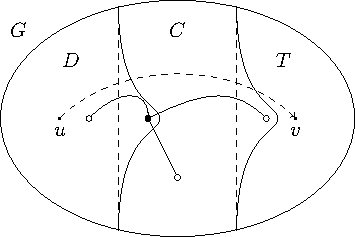
\includegraphics{./img/complexity_intro/GraphVisit.pdf}
    \end{center}
    \caption{Rappresentazione grafica dello schema di algoritmo di visita}
    \label{GraphVisit}
\end{figure}

La complessità è lineare nel numero degli archi. Tutti gli archi devono essere visitati almeno una
volta, se vogliamo fare una visita completa.

Tanti algoritmi di visita possono essere visti come modifiche di questo algoritmo qui andando a
lavorare su come viene gestita l'aggiunta di nuovi nodi a Current. Se si aggiunge in cima
si ha una politica in profondità (LIFO). Nel caso duale si ha una visita in larghezza. Queste sono
fondamentalmente le uniche due visite che hanno senso.

Visita in profondità e larghezza hanno caratteristiche diverse. La visita in profondità non
garantisce di trovare il cammino di lunghezza minima, quella in larghezza invece permette di trovare
sempre il cammino di lunghezza minima che collega il mio nodo di partenza ad un altro nodo del
grafo. La ricerca di un cammino minimo tra due nodi è un'operazione semplice.

È semplice calcolare il cammino più lungo in un grafo? Se lo fosse potremmo controllare la sua
lunghezza. Se questa fosse uguale a $n$ allora avremmo anche un cammino hamiltoniano. La ricerca di
un cammino lungo è quindi equivalente alla ricerca di un cammino hamiltoniano. E quindi è anche un
problema $\NPClass$-completo (lo vedremo più avanti).

In un certo senso il duale di un problema semplice è un problema difficile (cammino minimo vs.
cammino massimo). Non basta una semplice scansione dei cammini per trovare il più lungo, ma bisogna
considerarli tutti. Questo rende più complessa la ricerca.

Cercare cammini brevi è un'operazione facile, cercare cammini lunghi è difficile.

\section{Analisi di problemi}

Quando abbiamo un problema dobbiamo innanzitutto trovare un algoritmo stupido per dare un primo
upper bound alla complessità del problema. Gli algoritmi stupidi in genere fanno ricerche
esaustive. L'algoritmo stupido aiuta a cominciare a comprendere il problema.

Ad esempio, per trovare il cammino più lungo possiamo scansionare tutti i cammini semplici e dire
qual è il più lungo. Che upper bound abbiamo? Supponiamo di avere un grafo completamente connesso.
Possiamo calcolare il numero di cammini con tutte le permutazioni possibili tra $u$ e $v$. Abbiamo
quindi un numero fattoriale di cammini rispetto al numero dei nodi, e di conseguenza rispetto alla
dimensione del grafo. Questa complessità è dell'ordine di $n^{n}$: $n! \sim n^{n}$. 

Un grafo completamente connesso rappresenta un caso particolarmente sfavorevole. Tuttavia anche per
i grafi sparsi abbiamo un numero notevole di cammini. Tipicamente il numero è esponenziale o più
che esponenziale. Ad esempio in un grafo come quello della figura \ref{PathsNumber} abbiamo un
numero di archi che è lineare nell'ordine dei nodi ma abbiamo comunque un numero esponenziale di
cammini tra due nodi.

\begin{figure}[h]
    \begin{center}
        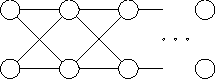
\includegraphics{./img/complexity_intro/ExponentialPathsNumber.pdf}
    \end{center}
    \caption{Esempio di grafo ``semplice'' con un grande numero di cammini possibili}
    \label{PathsNumber}
\end{figure}

La ricerca esaustiva è costosa. In linea di massima potremmo dare lo stesso upper bound per la
ricerca di cammini minimi. In realtà per fortuna con la ricerca breadth-first possiamo visitare i
nodi in ``ordine di distanza''. In questo modo possiamo individuare in maniera semplice i cammini
minimi. È quasi un miracolo in considerazione dello spazio di ricerca delle soluzioni di dimensione
esponenziale che abbiamo. 

Accade spesso che algoritmi polinomiali derivino dal fatto che invece di una ricerca esaustiva
possiamo farne una più mirata, grazie a particolari condizioni e risultati.

L'altro test semplice che si deve sempre fare è: ``data una soluzione esiste un modo semplice per
verificare che una soluzione sia corretta in modo efficace''? È possibile ``certificare'' in maniera
semplice una soluzione?

Il certificato per un cammino massimo non è banale: come facciamo a verificare che sia davvero il
massimo in maniera efficiente? Viceversa è invece banale il certificato per un cammino di lunghezza
$k$. Questo ammmette una verifica semplice, e questo colloca il problema di cercare un cammino di
lunghezza $k$ tra due nodi in un grafo in $\NPClass$, che è una classe piccola di problemi
esponenziali.

Una volta che abbiamo capito che sta in $\NPClass$ possiamo passare a chiederci se sta anche in
$\PClass$ e cominciare la ricerca di un algoritmo efficiente.

\subsection{Colorabilità}

Un altro problema interessante sui grafi è la colorabilità: capire se un dato grafo è colorabile con
$n$ colori. La ``difficoltà'' del problema problema dipende dal valore di $n$. La bicolorabilità di
un grafo è un problema semplice. Non tutti i grafi sono bicolorabili (vedi Figura
\ref{TwoColorableGraphs}). Un grafo può essere bicolorabile in più di un modo, a seconda di quale
colore scegliamo per iniziare la colorazione. Tuttavia questo non è un problema, dato che possiamo
sempre passare da una colorazione all'altra semplicemente complementando i colori.

\begin{figure}[h]
    \begin{center}
        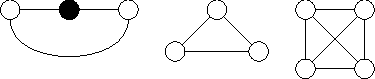
\includegraphics{./img/complexity_intro/2ColorableGraphs.pdf}
    \end{center}
    \caption{Esempi di grafi bicolorabili e di grafi non bicolorabili}
    \label{TwoColorableGraphs}
\end{figure}

Se abbiamo una cricca di dimensione $n$ abbiamo bisogno di almeno $n$ colori per colorarla, se
questa è in effetti colorabile. La colorabilità di un grafo è legata alla densità degli archi del
grafo.

La bicolorabilità è facilmente risolvibile mediante una visita. Il procedimento è a grandi linee
questo:
\begin{itemize}
    \item Ci poniamo la seguente invariante: i nodi già visitati e i nodi nella frontiera sono già
    stati colorati. Coloriamo quando aggiungiamo alla frontiera;
    \item Nella frontiera corrente selezioniamo un nodo;
    \item Andiamo a guardare i nodi connessi al corrente e facciamo la verifica di coerenza:
    \begin{itemize}
        \item Per ogni arco che ci riporta in Done verichiamo che i colori siano diversi, altrimenti
        ci blocchiamo. Questo perché il colore è forzato, se troviamo un'incoerenza non è
        possibile procedere altrimenti;
        \item Facciamo lo stesso controllo in Current.
    \end{itemize}
    \item Per i nodi in Todo li spostiamo in Current, assegnandoli un colore. Quale? Il colore
    complementare del current.
\end{itemize}

Se l'algoritmo arriva a termine senza bloccarsi il grafo è bicolorabile.

\begin{figure}[h]
    \begin{center}
        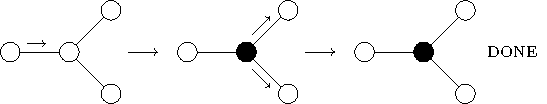
\includegraphics{./img/complexity_intro/2Coloration.pdf}
    \end{center}
    \caption{Esempio di bicolorazione di un grafo}
\end{figure}

Possiamo svolgere questo processo in una sola passata. Come mai? Perché l'assegnazione di colore è
univoca. Questo non è il caso con più di due colori: con tre colori potremmo scegliere tra due
alternative, e dovremmo fare backtracking. Il backtracking può portare (e in genere porta) ad
un'esplosione esponenziale.

Già la 3-colorabilità è un problema $\NPClass$-completo. Perché sta in $\NPClass$? Perché è
facile verficare la correttezza della colorazione, con una semplice visita arbitraria. $\NPClass$ è
una classe ragionevolmente vicina a $\PClass$.

\subsection{Problemi di flusso}

Una classe di problemi tipici sui grafi è quella dei problemi di flusso.

\begin{defn}
    Una rete $N$ è un grafo orientato con una sorgente $s$, un pozzo $t$ e una capacità $c(u,v)$
    associata ad ogni arco.
\end{defn}

\begin{defn}
    Un flusso in $N$ è una funzione $f(u,v)$ che ad ogni arco $(u,v)$ associa un intero positivo
    tale che
    \begin{itemize}
        \item $f(u,v) \leq c(u,v)$;
        \item la somma dei flussi entranti in ogni nodo (esclusi $s$ e $t$) è uguale alla
        somma dei flussi uscenti.
    \end{itemize}
\end{defn}

Il problema del flusso massimo è capire qual è il flusso massimo che la rete supporta, ovvero il
flusso tale che la somma dei flussi uscenti da $s$ (o equivalentemente di quelli entranti in $t$)
sia massima. Ci chiediamo quanto ``fluido'' riusciamo a far passare dalla sorgente al target. Un
upper bound è dato dal minimo tra la somma delle capacità degli archi uscenti dalla sorgente e la
somma di quelli entranti nel target. È un'importante ipotesi che le capacità siano intere.

%Noi vedremo un algoritmo semplice pensato per un caso particolare e una data complessità.
Vediamo un algoritmo semplice per risolvere il problema.

Per risolvere il problema inizialmente cerchiamo dei flussi banali, ovvero dei flussi lineari: la
quantità di fluido si incanala lungo un unico cammino. Quello che cerchiamo quindi è un cammino
qualunque tra sorgente e target. Lungo quel cammino cerchiamo di capire quanto fluido riusciamo a
far passare. Questo è limitato dalla capacità dell'arco di capacità minima nel cammino. Di
conseguenza definiamo un flusso che faccia uscire questa quantità di fluido dalla sorgente e la
faccia entrare nel target lungo il cammino.

Si procede in questo modo finché non ci sono più cammini tra $s$ e $t$, con l'accorgimento di fare
degli ``aggiustamenti'' alla rete legati al fatto che su alcuni archi stiamo già facendo passare del
flusso. Un'operazione è quella di diminuire la capacità di un arco lungo cui stiamo facendo già
passare del fluido, un'altra è quella di diminuire il fluido lungo un arco per farlo passare lungo
un altro.

L'algoritmo è dimostrabilmente corretto; andiamo quindi a discutere la complessità computazionale
dell'algoritmo.

La ricerca di flussi e la somma di flussi sono operazioni lineari nella dimensione del grafo.

Quante iterazioni faremo al massimo? Con ogni operazione diminuiamo almeno di uno il flusso massimo
che passa attraverso la rete. Usando gli upper bound sul flusso massimo dati prima abbiamo un
upper bound alle iterazioni.

Più formalmente procediamo per maggiorazioni. Indichiamo la capacità massima degli archi nel grafo
con $C$. Se supponiamo che tutti gli archi abbiano quella capacità abbiamo un upper bound $nC$ al
flusso massimo. La complessità delle operazioni di ricerca del flusso e applicazione del flusso è
$n^{2}$, quindi abbiamo una complessità dell'ordine $O(n^{3}C)$. È una complessità polinomiale?  No,
$C$ è un numero. In complessità bisogna stare attenti, specie quando abbiamo queste strutture
etichettate. La complessità dovrebbe essere un logaritmo di $C$ se volessimo un algoritmo
polinomiale. In effetti esistono casi patologici che fanno esplodere la complessità per via di $C$.

Data questa considerazione il nostro algoritmo non è polinomiale. Da ricordare è che se la
dimensione dei numeri è logaritmica, la complessità deve essere lineare nella dimensione dei dati.

Possiamo migliorare l'algoritmo? Sì, facendo una ricerca di cammino minimo quando andiamo a cercare
dei flussi. In questo caso la complessità diventa polinomiale. Possiamo risolvere il problema del
flusso massimo in tempo polinomiale.

\section{Problemi decisionali}

Un altro concetto importante è la differenza tra problemi di ottimizzazione e problemi di
decisione. Nel caso del flusso massimo abbiamo un problema di ottimizzazione. Abbiamo dei vincoli e
cerchiamo la soluzione minima (o massima) che soddisfa tali vincoli. In teoria della complessità
siamo interessati a problemi decisionali, ovvero con soluzione booleana Sì/No.

In un certo senso possiamo vedere i problemi di ottimizzazione come dei particolari problemi di
decisione, specie per i problemi di ottimizzazione discreti. Il trucco è, invece di chiederci se
esiste un flusso massimo, ci chiediamo ``esiste un flusso maggiore di $n$?''. È un problema meno
informativo, ma se sappiamo risolvere il problema decisionale possiamo pensare ad un algoritmo
efficiente per risolvere il problema di ottimizzazione. Ad esempio potremmo creare un loop che
esegue il nostro algoritmo per il problema decisionale per valori diversi dell'input finchè non
troviamo il massimo o minimo. Questo tuttavia non è molto astuto come metodo, ne esistono di
migliori.

Di solito risolvendo il problema di ottimizzazione non abbiamo la soluzione in sè, ma un valore
numerico tramite cui possiamo risalire alla soluzione in modo agevole. In altri termini otteniamo la
$x$ invece che la $f(x)$. Ma la $f$ è facilmente calcolabile, di conseguenza questo non è un
problema. Nel caso del problema del flusso massimo di solito la soluzione che otteniamo è il flusso,
non il suo valore. Tuttavia questo è facilmente calcolabile con la somma dei valori del flusso
sugli archi uscenti dalla sorgente, ad esempio.

Restringersi a problemi decisionali non è una decisione problematica, ed è interessante a livello
matematico. Perciò in complessità di solito si fa questa assunzione. Per noi il problema della
cricca sarà ``questo grafo ha una cricca di dimensione $k$?''.

\section{Problemi e linguaggi}

Nel problema decisionale abbiamo delle stringhe che descrivono l'input, in un qualche alfabeto.  Per
alcune stringhe la risposta al problema sarà Sì, per altre No. Il problema ci dà quindi un
linguaggio di stringhe che rappresentano input per cui la soluzione è Sì. La teoria della
complessità si può ridurre al problema di riconoscere stringhe di un linguaggio. L'algoritmo di
decisione del problema può essere visto come un algoritmo di riconoscimento del linguaggio delle
stringhe corrette. Le classi di complessità saranno quindi insiemi di linguaggi riconoscibili da
una macchina di Turing deterministica o meno con una data complessità.  Gli insiemi di linguaggi
sono pensati senza un'architettura specifica in mente.

\section{Riduzioni}

Un'altra problematica importante in Complessità e il problema della riduzione. Lo vediamo guardando
il problema del matching bipartito.

\subsection{Matching bipartito}

\begin{defn}
    Un grafo bipartito è una tripla $B = (U,V,E)$ dove $U$ e $V$ sono insiemi di uguale
    cardinalità e $E \subseteq U \times V$ è un insieme di archi.
\end{defn}

\begin{defn}
    Un matching per un grafo bipartito $B = (U,V,E)$ è un insieme $M \subseteq E$ che associa ad
    ogni elemento in $U$ uno e un solo elemento in $V$.
\end{defn}

Un grafo può essere suddiviso, a livello dei nodi, in due insiemi, tipicamente dalla stessa
cardinalità, i cui elementi non sono collegati. Otteniamo così un grafo bipartito.

Il problema del matching bipartito consiste nello stabilire se per un grafo bipartito esista o meno
un matching.

Non per tutti i grafi bipartiti esiste un accoppiamento, e non è del tutto ovvio come van create le
coppie.

Come lo risolviamo? Un approccio possibile è quello di sfruttare un algoritmo già noto e corretto
per un altro problema simile. Nel nostro caso possiamo sfruttare l'algoritmo per il problema del
flusso massimo. L'idea è che possiamo ridurre il problema del matching bipartito ad un problema di
flusso massimo.

Per fare ciò facciamo la seguente trasformazione al grafo bipartito $B = (U,V,E)$, ottenendo quindi un grafo
$B'$:
\begin{itemize}
    \item aggiungiamo un nodo $s$ ed un nodo $t$;
    \item aggiungiamo un arco da $s$ ad ogni nodo in $U$;
    \item aggiungiamo un arco a $t$ da ogni nodo in $V$;
    \item assegnamo ad ogni arco una capacità unitaria.
\end{itemize}

A questo punto per $B$ esiste un matching bipartito se e solo se $B'$ ammette un flusso massimo di
entità $n = |U| = |V|$, ovvero tale che il flusso totale uscente da $s$ sia uguale a $n$.

Questo è un tipico esempio di riduzione. Abbiamo un problema, il matching bipartito, e lo riduciamo
ad un altro problema, che sappiamo già risolvere. Utilizziamo il problema del flusso massimo per risolvere
il nuovo problema. Che operazione facciamo per fare ciò? L'unica cosa che facciamo è trasformare
i dati di input in una rete di flusso. Dopodiché li diamo in input all'algoritmo per il flusso
massimo. In base alla risposta del primo abbiamo automaticamente la risposta del secondo.

\begin{figure}[h]
    \begin{center}
        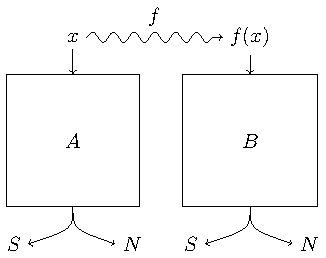
\includegraphics{./img/complexity_intro/Reducibility.pdf}
    \end{center}
    \caption{Schema di riduzione di un problema $A$ in un problema $B$}
\end{figure}

La tentazione di solito è quella di cambiare un algoritmo per adattarlo ad un nuovo problema. In
questo caso non facciamo quello; noi prendiamo i dati di input e li trasformiamo in modo che
l'algoritmo iniziale lo possa accettare. L'algoritmo rimane lo stesso, quello che viene adattato è
l'input. Questo significa fare una riduzione.

Avremo però qui dei vincoli in più rispetto alla riduzione della teoria della calcolabilità. Ad
esempio avremo vincoli sul costo computazionale di $f$. Qui è in un certo senso più intuitivo
rispetto alla teoria della calcolabilità, dato che facciamo trasformazioni da strutture dati a
strutture dati (che per noi sono sempre stringhe), mentre in teoria della calcolabilità si
trasformano numeri in numeri.

Esiste un'altra nozione di riducibilità, la Turing riducibilità. Immaginiamo un oracolo che risolve
$B$ e che possiamo interrogare quante volte vogliamo. Possiamo ora risolvere un dato problema $A$?
In questo caso avremmo che $A$ è Turing-riducibile a $B$.

Per quanto riguarda il concetto di riduzione possiamo pensare ad un problema $A$ e ad un problema
$B$ come linguaggi. Con una riduzione da $A$ a $B$ abbiamo che $x \in A \iff f(x) \in B$. Questa è una
nozione di riducibilità, ce ne sono altre più potenti.

\subsection{Riducibilità e classi di complessità}

La riducibilità è interessante ai fini della complessità. Supponiamo di avere una classe di
complessità $\CClass$ e supponiamo che $B \in \CClass$. Se riusciamo a ridurre $A$ a $B$ vorremmo
poter concludere che anche $A \in \CClass$.

Per fare ciò è importante prendere una nozione di riducibilità abbastanza fine per le classi a
cui siamo interessanti. Una riduzione troppo forte, come la Turing-riducibilità, potrebbe dare
problemi.

Ad esempio pensiamo di poter complementare la risposta di un oracolo. In questo caso potremmo
ridurre ogni linguaggio al suo complementare, che non è sempre quello che vogliamo. Potremmo non
essere in grado di osservare differenze tra classi con una nozione così forte, mentre con una più
debole (o fine) possiamo osservare certe differenze. Con riduzioni forti le classi in un certo senso
collassano. Questo è interessante se vogliamo studiare classi di complessità (o linguaggi) che non
sono chiuse per complementazione.

\begin{figure}[h]
    \begin{center}
        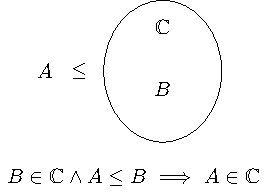
\includegraphics{./img/complexity_intro/ReducibilityNotion.pdf}
    \end{center}
    \caption{Chiusura di classi di complessità in base alla nozione di riducibilità}
    \label{ReducibilityNotion}
\end{figure}

Tutte le classi non deterministiche non sono chiuse per complementazione (come non lo erano insiemi
r.e.). Ad esempio i complementari di linguaggi in $\NPClass$ stanno in $\CONPClass$. In questo caso
non ha senso usare una nozione troppo forte di riducibilità.

Concludere l'appartenenza di $A$ in una classe $\CClass$ in base alla sua riducibilità ad un
problema $B$ in $\CClass$ non è immediato e dipende dalla nozione di riducibilità. In particolare
andrà dimostrato.

\subsection{Complessità di $f$}

La nozione di base di riducibilità l'abbiamo data, ma non basta. Si pongono dei limiti su $f$: si
richiede che $f$ abbia complessità polinomiale in tempo. Questo perché vogliamo che valga la
proprietà di chiusura della figura \ref{ReducibilityNotion}. Infatti se risolviamo $B$ in tempo
polinomiale e $f$ opera una trasformazione anch'essa polinomiale in tempo, componendo i due
algoritmi avremmo un nuovo algoritmo polinomiale in tempo per risolvere $A$.

Richiedere che $f$ sia addirittura lineare sarebbe più fine di quanto ci interessa: sarebbero troppi
pochi i problemi riducibili ad un dato problema. Un vincolo polinomiale sembra essere abbastanza
ragionevole.  Ammettere funzioni di riduzione esponenziali permetterebbere di ridurre
fondamentalmente qualsiasi problema a qualsiasi altro.

Problemi che appartengono apparentemente a domini completamente diversi possono essere agevolmente
ridotti l'uno all'altro. Ad esempio $\SAT$ è riducibilie alla copertura di vertici di un grafo. La
soddisfacibilità è stato il primo problema ad essere stato dimostrato essere $\NPClass$-completo. Se
abbiamo un problema $A$ che è $\NPClass$-completo e abbiamo $B$ tale che $A \leq B$ diremo che $B$
è $\NPClass$-hard.

Le riduzioni aiutano a vedere i problemi in un modo diverso dal solito.

Vediamo alcuni esempi di riduzioni polinomiali tra problemi.

\subsection{Colorabilità}

Vediamo ora che la $n$-colorabilità e riducibile alla $n+1$-colorabilità: $n\textsc{-color} \leq
n+1\textsc{-color}$.

Cosa prende in input $n$\textsc{-color}? Un grafo e dice se è $n$ colorabile. Fissiamo $n$ a 3 e dimostriamo
che $3\textsc{-color} \leq 4\textsc{-color}$.

Possiamo fare la riduzione con la nozione di riducibilità che abbiamo visto prima?

Bisogna fare attenzione a ``non dare per ovvia la soluzione''. Ad esempio è pressocchè sempre
sbagliato pensare che la funzione di riduzione sia l'identità, dato che l'identità solitamente
permette solo di ridurre un linguaggio a se stesso. In questo caso avremmo un verso ma non avremmo
l'altro: un grafo 3-colorabile è sicuramente 4-colorabile ma non vale il viceversa, il che è
importante per la riduzione.

Cosa dobbiamo fare? Dobbiamo prendere il grafo $G$ in input per 3\textsc{-color} e trasformarlo in
un grafo $G'$ che soddisfi la condizione di riduzione. Prendiamo $G$ e aggiungiamo un nodo che
colleghiamo a tutti i nodi di $G$. Per poter colorare questo nodo abbiamo bisogno di un colore nuovo
non in $G$.  Se $G$ è 3-colorabile allora $G'$ è 4-colorabile. Viceversa se $G'$ è 4-colorabile
il colore usato dal nodo aggiunto deve essere diverso da quello dei nodi del sottografo che
corrisponde a $G$, che quindi risulta 3-colorabile.

\begin{figure}[h]
    \begin{center}
        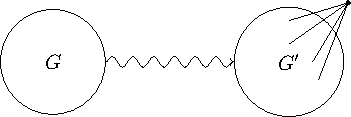
\includegraphics{./img/complexity_intro/3COL4COL.pdf}
    \end{center}
    \caption{Riduzione del problema della $n$-colorabilità alla $n+1$-colorabilità}
\end{figure}

\subsection{Cricca e insieme indipendente}

Vediamo un altro esempio. Proviamo a ridurre il problema dell'insieme indipendente al problema della
cricca: $\textsc{is} \leq \textsc{cricca}$.

L'input di \textsc{is} è una coppia $(G,k)$ e ci chiediamo se esista un insieme indipendente di
dimensione $k$. L'input di CRICCA è una coppia $(G,k)$ e chi chiediamo se esista una cricca di
dimensione $k$.

La trasformazione è semplice: complementiamo il grafo. Dove c'era un insieme indipendente di nodi
avremo tutti i collegamenti possibili tra di essi, e quindi una cricca.

\section{Ricerca vs. Verifica}

%// TODO
%Slide 40

Un conto è cercare una soluzione, un conto è verificare la correttezza di una soluzione.

Di nuovo, quando incontriamo un problema bisogna pensare innanzitutto all'algoritmo stupido di
ricerca esaustiva.

%La complessità dell'algoritmo stupido per l'insieme indipendente è polinomiale per $k$ fissato. Se $k$
%però fa parte del'input questo non è più necessariamente vero. Con $k \in O(n)$ abbiamo un
%algoritmo esponenziale.

Non sempre il certificato è una soluzione al problema. È un'informazione in più che ci viene data e
che ci permette di verificare in modo agevole la correttezza di una data soluzione. Non per tutti i
problemi è possibile effettuare la verifica in tempo polinomiale (e.g. torri di Hanoi).

$\NPClass$ è una classe interessante perché contiene problemi facilmente certificabili.

\section{Relazioni tra alcune classi di complessità}

Cosa significa $A \in \NPClass$? Significa che $\exists B \exists p, B \in \PClass \land p\textit{ polinomio}$
tale che
\begin{equation*}
    x \in A \iff \exists c_{x}, |c_{x}| \leq p(x) \land \pair{x}{c_{x}} \in B
\end{equation*}

La seconda parte dello statement ci dice che possiamo verificare che $c_{x}$ è un buon certificato per
$x$ in tempo polinomiale. La prima parte dice che il certificato deve avere dimensione polinomiale.

Il linguaggio delle coppie $\pair{x}{c_{x}}$ deve far parte di $B$ sse $x \in A$. 

C'è una differenza tra parlare di linguaggi e di macchine. Un linguaggio appartiene ad una certa
classe se esiste una MdT che lo riconosce secondo le condizioni della classe, ma non è la macchina
a far parte della classe. Le classi di complessità comprendono linguaggi, non macchine.

Per tanti problemi possiamo certificare la correttezza con un certificato, per altri no. Ad esempio
per la soddisfacibilità si può fare, per la tautologicità no. Il problema è la dimensione del
certificato.

Per tutti i problemi abbiamo un algoritmo generate and test, il problema sta nella ricerca che è
costosa.

%// TODO
%Slide 43

Ci sono alcuni problemi in $\NPClass$ di cui non si è dimostrata la completezza ma di cui se si potesse
dimostrare l'incompletezza avremmo $\PClass \not= \NPClass$. Finora non si è dimostrata l'incompletezza di
nessun problema in $\NPClass$.

%A volte è possibile verificare che una soluzione sia corretta mediante un certificato ma potrebbe
%non essere possibile verificare che una solzuione si scorretta (sempre mediante certificato)

Si congettura la gerarchia di classi di complessità mostrata in figura \ref{ConjecturedHierarchy}.

\begin{figure}[h]
    \begin{center}
        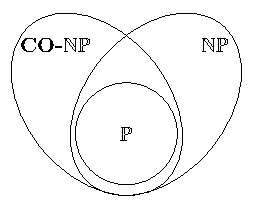
\includegraphics{./img/complexity_intro/NPCONP.pdf}
    \end{center}
    \caption{Gerarchia congetturata di alcune classi di complessità}
    \label{ConjecturedHierarchy}
\end{figure}

Si congettura che $\NPClass$ sia diverso da $\PClass$, e che l'intersezione tra $\CONPClass$ e
$\NPClass$ sia diversa da $\PClass$. Abbiamo che $\COPClass$ è uguale a $\PClass$. Se si dimostra,
come si congettura, che $\COPClass$ sia diverso da $\CONPClass$ allora avremmo anche che $\NPClass$
sarebbe diverso da $\PClass$. Se si dimostra $\PClass = \NPClass$ allora
collasserebbero tutte su $\PClass$. Abbiamo inoltre che ogni problema non banale in $\PClass$ è
$\PClass$-completo. Se si dimostrasse che esiste un problema in $\NPClass$ incompleto avremmo
$\PClass \not= \NPClass$.

Un problema molto studiato è quello dell'isomorfismo tra grafi. Il problema è capire se due grafi
$G,G'$ sono isomorfi, ovvero hanno la stessa struttura topologica. È un problema che ha un sacco di
applicazioni concrete.

Possiamo certificare una soluzione per questo problema? Sì, con il mapping usato. Il numero di mapping
è esponenziale, perciò una ricerca esaustiva non è un granché. Di solito si cerca di pilotare la
ricerca in modo da renderla più veloce, ad esempio sapendo che certi nodi non possono essere
mappati in certi altri in base a certe condizioni.

Si congettura che questo problema, in questa forma, non sia completo. Non se ne è ancora dimostrata
la completezza. C'è un problema simile, che è quello dell'isomorfismo di sottografo. Quello è un
problema completo. Questo perché generalizza il problema della cricca.

Vediamo un problema che sta in $\CONPClass \cap \NPClass$ che si congettura non essere completo
(altrimenti collasserebbe tutto).

Questo problema è la fattorizzazione di un numero intero. La versione decisionale prende $(n,k)$ e
ci chiediamo se $n$ è fattorizzabile con meno di $k$ fattori. Sta in $\NPClass$? Sì. Non è banale
perché fino a poco tempo fa non si sapeva se il test di primalità fosse polinomiale. Ma sappiamo
ora che lo è, quindi la verifica della fattorizzazione è semplice.

Abbiamo un certificato per dire che un numero non è fattorizzabile in meno di $k$ fattori? Sì,
sempre la fattorizzazione. Questo perché la fattorizzazione è unica.

Il certificato va bene per entrambi i casi, basta cambiare il metodo di verifica.
